\documentclass[a4paper]{article}

% CUSTOM maketitle
\makeatletter
 \def\@maketitle{%
  \newpage
  \null
  \vskip 1.em
  \begin{center}%
  \let \footnote \thanks
    {\LARGE \bfseries\@title \par}%
    \vskip 1.em%
    {\large \langCourse \par}%
     {\large \langInstitute \par}%
    \vskip 1.em%
    {\large
      \lineskip .5em%
      \begin{tabular}[t]{c}%
        \@author { --- } \@istid \\
        {\href{mailto:\@email}{\tt\@email}}
      \end{tabular}\par}%
          \vskip 1.em%
    \ifx\@coadvisor\undefined      
        {\large \langAdvisor: \@advisor \par}%
    \else
        {\large \langAdvisor: \@advisor \par}%
        {\large \langCoadvisor: \@coadvisor \par}%
    \fi
    
  \end{center}%
  \par
  \vskip 1em}
\makeatother


% Commands to allow defining title, name, etc.
\makeatletter
\newcommand{\@StoreIn}[2]{ \gdef#1{#2} }
\newcommand*{\email}[1]{\@StoreIn{\@email}{#1}}
\newcommand*{\istid}[1]{\@StoreIn{\@istid}{#1\thanks{\langThanks}}}
\newcommand*{\advisor}[1]{\@StoreIn{\@advisor}{#1}}
\newcommand*{\coadvisor}[1]{\@StoreIn{\@coadvisor}{#1}}
\makeatother

% The 'utf8' package contains support for using UTF-8 as input encoding. 
\usepackage[utf8]{inputenc}
% The 'babel' package may correct some hyphenation issues of LaTeX. 
% Select your MAIN LANGUAGE for the Thesis with the 'main=' option.
\usepackage[english]{babel}
\usepackage{iflang}

% Solves some font enconding issues related to the output
\usepackage[T1]{fontenc}

% These packages are typically required. 
% Among many other things they add the possibility to put symbols in bold
% by using \boldsymbol (not \mathbf); defines additional fonts and symbols;
% adds the \eqref command for citing equations.
\usepackage{mathtools, amsmath, amsthm, amssymb, amsfonts}
\usepackage{nicefrac}
%

% Tikz  for creating graphics programmatically.
\usepackage{tikz}
\usetikzlibrary{shapes.geometric, arrows, positioning}

% These packages are most usefull for advanced tables. 
% 'multirow' allows to join rows throuhg the command \multirow which works
% similarly with the command \multicolumn.
% The 'colortbl' package allows to color the table (foreground and background)
% The package 'booktabs' provide some additional commands to enhance
% the quality of tables
% The 'longtable' package is only required when tables extend beyond the length
% of one page, which typically does not happen and should be avoided
\usepackage{array}
\usepackage{booktabs}
\usepackage{multirow}
\usepackage{colortbl}
\usepackage{spreadtab}
\usepackage{longtable}
\usepackage{pdflscape}
\usepackage{float}

% Set links for references and citations in document
\usepackage{hyperref}
\hypersetup{ colorlinks=true,
             citecolor=cyan,
             linkcolor=darkgray,
             urlcolor=teal,
             breaklinks=true,
             bookmarksnumbered=true,
             bookmarksopen=true,
}

% Provides better support for handling and breaking URLs.
\usepackage{url} 

% The package 'graphicx' supports formats PNG and JPG.
% Package 'subfigure' allows to place figures within figures with own caption. 
% For each of the subfigures use the command \subfigure.
\usepackage{graphicx}
\usepackage[hang,small,bf,tight]{subfigure}

\usepackage[format=hang,labelfont=bf,font=small]{caption} 
% the following customization adds vertical space between caption and the table
%\captionsetup[table]{skip=10pt}

% These packages are required for list code snippets.
\usepackage{xcolor}
\usepackage{color}
% The following special color definitions are used in the IST Thesis
\definecolor{forestgreen}{RGB}{34,139,34}
\definecolor{orangered}{RGB}{239,134,64}
\definecolor{lightred}{rgb}{1,0.4,0.5}
\definecolor{orange}{rgb}{1,0.45,0.13}	
\definecolor{darkblue}{rgb}{0.0,0.0,0.6}
\definecolor{lightblue}{rgb}{0.1,0.57,0.7}
\definecolor{gray}{rgb}{0.4,0.4,0.4}
\definecolor{lightgray}{rgb}{0.95, 0.95, 0.95}
\definecolor{darkgray}{rgb}{0.4, 0.4, 0.4}
\definecolor{editorGray}{rgb}{0.95, 0.95, 0.95}
\definecolor{editorOcher}{rgb}{1, 0.5, 0} % #FF7F00 -> rgb(239, 169, 0)
\definecolor{chaptergrey}{rgb}{0.6,0.6,0.6}
\definecolor{editorGreen}{rgb}{0, 0.5, 0} % #007C00 -> rgb(0, 124, 0)
\definecolor{olive}{rgb}{0.17,0.59,0.20}
\definecolor{brown}{rgb}{0.69,0.31,0.31}
\definecolor{purple}{rgb}{0.38,0.18,0.81}

%For enhanced enumeration of lists
%\usepackage{enumitem}
\usepackage[shortlabels]{enumitem}
\setlist[description]{leftmargin=\parindent,labelindent=\parindent,itemsep=1pt,parsep=0pt,topsep=0pt}

% For rotating
\usepackage{rotating}
% For Gantt chart generation
\usepackage{pgfgantt}
% For dummy text generation
\usepackage{lipsum} 

% To define margins to be OF THE SAME DIMENSIONS AS DEI MASTER TEMPLATE
\usepackage{geometry}
\geometry{ 
  a4paper,         
  inner=1in,
  outer=1in,
  headheight=16pt,
  % textheight=637pt, 
  % textwidth=455pt,
  marginparsep=0pt,
  headsep=25pt,
  top=106pt,
  marginparwidth=56pt,
    heightrounded,   % integer number of lines
}

% The package 'acronym' garantees that all acronyms definitions are 
% given at the first usage. 
% IMPORTANT: do not use acronyms in titles/captions; otherwise the definition 
% will appear on the table of contents.
\usepackage[printonlyused]{acronym}

% BIBLIOGRAPHY related packages
\usepackage{cite}
\bibliographystyle{IEEEtran}
\usepackage{ulem}


% TITLE related packages  
\usepackage[runin]{abstract}

% To insert good looking code
\usepackage{listings}
\lstdefinestyle{mystyle}{
    backgroundcolor=\color{white},   % choose the background color
    basicstyle=\ttfamily\small,      % the size of the fonts used for the code
    breakatwhitespace=false,         % sets if automatic breaks should only happen at whitespace
    breaklines=true,                 % sets automatic line breaking
    captionpos=b,                    % sets the caption-position to bottom
    commentstyle=\color{green!40!black},  % comment style
    keywordstyle=\color{blue},       % keyword style
    keywordstyle={[2]\color{purple!80!black}}, % additional keywords
    keywordstyle={[3]\color{orange}}, % additional keywords
    identifierstyle=\color{black},   % identifier style
    numberstyle=\tiny\color{gray},   % the style used for line-numbers
    numbers=left,                    % where to put the line-numbers
    numbersep=5pt,                   % how far the line-numbers are from the code
    stringstyle=\color{orange},      % string literal style
    showspaces=false,                % show spaces everywhere adding particular underscores
    showstringspaces=false,          % underline spaces within strings only
    showtabs=false,                  % show tabs within strings adding particular underscores
    tabsize=4,                       % default tabsize
    emph={int,char,double,float,unsigned,void},
    emphstyle={\color{blue}},
    emph={[2]for, while, do, if, else, switch, case},
    emphstyle={[2]\color{purple!80!black}},
    emph={[3]printf, scanf, cout, cin, endl, include},
    emphstyle={[3]\color{orange}}
}
% Use the defined style for code listings
\lstset{style=mystyle}

\colorlet{punct}{red!60!black}
\definecolor{background}{HTML}{EEEEEE}
\definecolor{delim}{RGB}{20,105,176}
\colorlet{numb}{magenta!60!black}

\lstdefinelanguage{json}{
    basicstyle=\normalfont\ttfamily,
    numbers=left,
    numberstyle=\scriptsize,
    stepnumber=1,
    numbersep=8pt,
    showstringspaces=false,
    breaklines=true,
    frame=lines,
    backgroundcolor=\color{background},
    literate=
     *{0}{{{\color{numb}0}}}{1}
      {1}{{{\color{numb}1}}}{1}
      {2}{{{\color{numb}2}}}{1}
      {3}{{{\color{numb}3}}}{1}
      {4}{{{\color{numb}4}}}{1}
      {5}{{{\color{numb}5}}}{1}
      {6}{{{\color{numb}6}}}{1}
      {7}{{{\color{numb}7}}}{1}
      {8}{{{\color{numb}8}}}{1}
      {9}{{{\color{numb}9}}}{1}
      {:}{{{\color{punct}{:}}}}{1}
      {,}{{{\color{punct}{,}}}}{1}
      {\{}{{{\color{delim}{\{}}}}{1}
      {\}}{{{\color{delim}{\}}}}}{1}
      {[}{{{\color{delim}{[}}}}{1}
      {]}{{{\color{delim}{]}}}}{1},
}


% Set language dependent texts
\newcommand{\keywords}[1]{\IfLanguageName{english}{\\[10pt]\textbf{{Keywords ---}} #1}{\\[10pt]\textbf{{Palavras Chave ---}} #1}}
\newcommand{\palavrasChave}[1]{\IfLanguageName{english}{\\[10pt]\textbf{{Palavras Chave ---}} #1}{\\[10pt]\textbf{{Keywords ---}} #1}}
\newcommand{\langAdvisor}{\IfLanguageName{english}{Advisor}{Orientador}}
\newcommand{\langCoadvisor}{\IfLanguageName{english}{Co-advisor}{Co-orientador}}
\newcommand{\langCourse}{\IfLanguageName{english}{Master in Computer Science and Engineering}{PIC2 - Mestrado em Engenharia Informática e de Computadores}}
\newcommand{\langInstitute}{\IfLanguageName{english}{Instituto Superior Técnico, Universidade de Lisboa}{Instituto Superior Técnico, Universidade de Lisboa}}
\newcommand{\langThanks}{\IfLanguageName{english}{I declare that this document is an original work of our own authorship and that it fulfills all the requirements of the Code of Conduct and Good Practices of the Universidade de Lisboa (\url{https://nape.tecnico.ulisboa.pt/en/apoio-ao-estudante/documentos-importantes/regulamentos-da-universidade-de-lisboa/}).}{Declaro que o presente documento é um trabalho original da minha autoria e que cumpre todos os requisitos do Código de Conduta e Boas Práticas da Universidade de Lisboa (\url{https://nape.tecnico.ulisboa.pt/en/apoio-ao-estudante/documentos-importantes/regulamentos-da-universidade-de-lisboa/}).}}

% Customize Table of Contents
\setcounter{tocdepth}{2} % Include subsections in TOC
\setcounter{secnumdepth}{3} % Number subsections

\usepackage{tabularx}


% Diagrams: https://mermaid.live/
% Tips for Writing Technical Papers: https://cs.stanford.edu/people/widom/paper-writing.html

\begin{document}

%%%%%%%%%%%%%%%%
% TITLE & NAME %
%%%%%%%%%%%%%%%%
\selectlanguage{english}
\title{E-Rocket Report 1 - Using PX4 hardware to read sensor data and actuate servos and motors}
\author{Pedro Maria da Costa Almeida Martins}
\istid{99303}
\email{pedromcamartins@tecnico.ulisboa.pt}
\advisor{Prof. Paulo Oliveira}
\coadvisor{Pedro Santos}

% To make the title
\maketitle
\thispagestyle{empty}
\clearpage


%%%%%%%%%%%%%%%%%%%%%
% TABLE OF CONTENTS %
%%%%%%%%%%%%%%%%%%%%%
\tableofcontents
% \listoffigures      % List of Figures
% \listoftables       % List of Tables
% \lstlistoflistings  % List of Listings
\thispagestyle{empty}
\clearpage



\section{Background}

One requirement of this system is to be able to run controllers developed by the team. 
To test if this is possible given the current setup, the team decided to start with a demonstration that read sensor data and used it to control the servos and motors. 

PX4 is an open-source flight control software that runs on a variety of hardware platforms.
It is designed to be used in drones, but it can also be used in other vehicles, such as cars and boats.
PX4 is a modular system, meaning that it can be extended to add new features.
It is composed of a set of modules that communicate with each other using a publish-subscribe model, with the help of a uOrb communication bus. 

PX4 currently doesn't provide native support for a drone with a TVC module. This means that the team cannot natively use some parts of the ecosystem. 
These includes simulators like gazebo, airframes, autonomous flight modes, existing controllers and navigation algorithms, and RC control. 
This constraint had to be taken into account when designing the system. 
% add links to the the PX4 documentation that shows these limitations

There are two major ways of extending the functionality of a vehicle running PX4: Modifying the firmware to add features (called modules), or to use an offboard computer to control PX4. 
The team decided to use an offboard computer, as it seemed simpler, faster and more intuitive. 
% add links to modifying the firmware and offboard computer documentation

To communicate with the PX4, the two options that PX4 provides are MAVLink and ROS2 interface. 
The team chose to use ROS2 interface, because MavLink although simpler to use, is limited to MAVLink services, meaning some needed information may not be exposed through it. 
Additionally, ROS2 is a more powerful framework, with a large ecosystem of packages and libraries. 
% add link to this https://docs.px4.io/main/en/robotics/

To validate if the demo works, we could either use simulation (as it is used in PX4 offboard controller example), or use the actual hardware. 
The team decided to validate the demo in the actual hardware, as we already had the functional hardware, and as mentioned before, there's no native support for our drone in the simulation.
% add link to the PX4 offboard controller example

In the final product, the offboard computer should be aboard the drone, but for convenience, a laptop was used. 
This should not affect the conclusions taken from this report, as both the laptop and the Raspberry Pi (used on the final product) use the same Operating Systems and packages. \\

In summary, the objectives of this demonstration is to: 

\begin{itemize}
    \item Use real hardware 
    \item Control servo and motor PWM signals. 
    \item Read sensor data, and be able to use it. 
\end{itemize}

This demo was accomplished by using the assembled TVC mechanism and connecting an offboard computer, which in this case was a Laptop running Linux. 



\section{Architecture}

%% insert software architecture image
%% insert hardware architecture image

The system is composed of two main components: the PX4 flight controller and the offboard computer. 
The PX4 flight controller is responsible for the hardware drivers, sensors readings, and position and attitude estimation. 
The offboard computer is responsible for reading the sensor data, and actuate the servos and motors. 

\subsection{PX4}

In order to control PX4, PX4 has to change its internal state machine mode to offboard.
In addition, the offboard computer has to send a heartbeat message to PX4, so that it knows that the offboard computer is connected.
If the offboard computer is not sending a specfic offboard mode message, PX4 will switch to the failsafe mode (configured as disarm mode).
% add link to https://docs.px4.io/main/en/flight_modes/offboard.html#ros-2-messages

To control the servos and motors, the offboard computer has to send a message, informing the level of the PX4 control architecture at which offboard setpoints must be injected, while disabling the bypassed controllers. 
In this case, the desired control quantity is direct motors and servos. 
% insert table in https://docs.px4.io/main/en/flight_modes/offboard.html#ros-2-messages
Afterwards, the offboard computer can send the desired PWM values to the motors and servos.

Due to PX4's safety features, the motors are only enabled when the vehicle is armed. 
This menas that the offboard computer has arm the vehicle before sending the PWM values to the motor. 

\subsection{uXRCE-DDS}

To connect PX4 to ROS2, PX4 uses uXRCE-DDS, which is a lightweight implementation of DDS. 
This acts as a middleware between the uOrb, used between modules in PX4, and the ROS2 topics, used between ROS2 nodes. 
To use uXRCE-DDS, a uXRCE-DDS client runs in PX4, and a uXRCE-DDS agent runs in the offboard computer. 
This is shown in the diagram below: 

\begin{figure}[H]
    \centering
    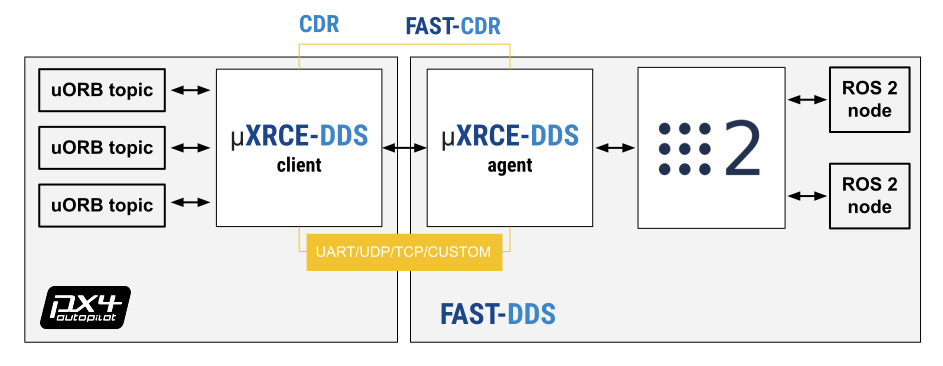
\includegraphics[width=0.8\textwidth]{imgs/architecture_xrce_dds_ros2.png}
    \caption{Software architecture connecting PX4 to ROS2 using uXRCE-DDS.}
    \label{fig:architecture_xrce_dds_ros2}
\end{figure}
% add link to the uXRCE-DDS documentation + image

In our case, the connection between client and agent is done using a serial connection. 

% mention the fact that not all of the messages are implemented... 

\subsection{ROS2}

ROS2 is a set of software libraries and tools that help you build robot applications.
It is a modular system, meaning that it can be extended to add new features.
It is composed of a set of nodes that communicate with each other using a publish-subscribe model, with the help of a DDS communication bus.

The offboard computer contains a ROS2 workspace, which is a set of packages that can be built and run together.
% add link to the ROS2 workspace in e-rocket repo

The demo workspace uses 3 packages: 
\begin{itemize}
    \item \verb|px4_msgs|: This package contains all the messages used by PX4, and a node that connects to the uXRCE-DDS agent, and subsctibes to the PX4 uOrb messages.
    \item \verb|offboard_control|: This package contains the offboard control node that subscribes to the sensor messages, and publishes the servo and motor messages.
    \item \verb|plot_juggler|: This package is used to visualize ROS2 topics and messages in real time, with the help of a GUI.
\end{itemize}



\section{Setup}

\subsection{PX4}

Before being able to test this demo, a number of configurations are required. 

\subsubsection{Firmware}

The first step when using hardware like PixHawk, which runs the PX4 software, is to flash the PX4 firmware. 
The team chose the latest stable version. 

\subsubsection{Airframe}

After installing firmware you need to select a vehicle type and frame configuration. 
This applies appropriate initial parameter values for the selected frame, such as the vehicle type, number of motors, relative motor position, and so on. 
% add link https://docs.px4.io/main/en/config/airframe.html

The team started by using a baloon frame, because the vehicle is uncontrolled (adeactivates the native flight controller algorithms). 
This turned out to not be the feasable, as this frame also disables the capacity to configure servos, which our system requires. 
Instead, the team used the generic multicopter frame, with a custom generic geometry. 
% add link 

\subsubsection{Servo setup}

Using a generic geometry, 2 motors and 2 servos were configured to the outputs. 
% TODO: add outputs (FMU aux, ...)

Note that PWM AUX outputs are preferred over the PWM MAIN outputs for controlling motors (as they have lower latency). 
% add link https://docs.px4.io/main/en/config/actuators.html#actuator-outputs

\subsubsection{Safety checks}

...

\subsubsection{uXRCE-DDS client setup}

The team followed the official tutorial 
% add link https://docs.px4.io/main/en/middleware/uxrce_dds.html#starting-the-client
TELEM 2 Serial Port was configured as the port used by the client. 

% Additional parameter configuration

\subsection{Offboard computer}

\subsubsection{uXRCE-DDS agent setup}

The team followed the official tutorial, and configured the agent to connect to the serial port where PixHaw was connected.
% add link https://docs.px4.io/main/en/middleware/uxrce_dds.html#starting-the-agent

\subsubsection{ROS2 setup}

The team followed the official tutorial, installing ROS2 humble edition on Ubuntu 20.04. 
% add link


\subsubsection{PX4 ROS2 messages}





\section{Demo}

The demo only uses sensor data from the attitude estimator, which uses the Extended Kalman Filter present in PX4. 
It was heavily inspired by the PX4 ROS2 examples. 
% add link to the px4_ros2_com repository

The demo uses the following messages: 

\begin{itemize}
    \item \verb|px4_msgs::msg::ActuatorMotors|: Sends PWM values to the motors.
    \item \verb|px4_msgs::msg::ActuatorServos|: Sends PWM values to the servos.
    \item \verb|px4_msgs::msg::SensorAttitude|: Gets the attitude data as a quaternion, from the attitude estimator.
    \item \verb|px4_msgs::msg::VehicleCommand|: Sends commands to PX4, such as arming and disarming the vehicle.
    \item \verb|px4_msgs::msg::VehicleControlMode|: Sends the control mode to PX4, such as offboard mode.
    \item \verb|px4_msgs::msg::OffboardControlMode|: Sends the control mode to PX4, such as direct motor and servo control.
\end{itemize}

The code consists of a Ros2 node that contains the main logic of the demo. 
It includes the subscribers/ publishers for the PX4 Messages, and auxiliary functions and variables. 
The constructor of the Ros2 node is executed once, when the node is created (using \verb|spin| function in main). 

The code includes two main callbacks, which means they get called to respond to an event. These callbacks include: 
\begin{itemize}
    \item The subscriber to the \verb|px4_msgs::msg::SensorAttitude| message, that is called when a new message is received. This function uses the attitude data to control the servos, and actuates the motors. 
    \item A timer callback function, which is called every 100ms by a software timer. 
\end{itemize}

\subsection{Demo Code}

\subsubsection{Class OffboardControl}

The class called \verb|OffboardControl| which extends the \verb|Node| class, is the main class of the demo. 
It contains the variables and functions used. 

The function \verb|OffboardControl()| is the constructor of the class, which initializes the node, the publishers, subscribers subscribers, and both routines: the timer and the attitude subscriber.

\begin{lstlisting}[language=C++, caption=Offboard control example]
class OffboardControl : public rclcpp::Node 
{
public:
    explicit OffboardControl() : Node("offboard_control");
private:
    rclcpp::TimerBase::SharedPtr timer_;

    rclcpp::Publisher<ActuatorMotors>::SharedPtr actuator_motors_publisher_;
    rclcpp::Publisher<ActuatorServos>::SharedPtr actuator_servos_publisher_;
    rclcpp::Publisher<VehicleCommand>::SharedPtr vehicle_command_publisher_;
    rclcpp::Publisher<OffboardControlMode>::SharedPtr offboard_control_mode_publisher_;
    rclcpp::Publisher<VehicleControlMode>::SharedPtr vehicle_control_mode_publisher_;
    rclcpp::Subscription<VehicleAttitude>::SharedPtr vehicle_attitude_subscription_;

    uint64_t timer_callback_iteration_ = 0;   //!< counter for the number of setpoints sent

    bool is_offboard_mode_ = false;

    std::atomic<float> roll_;   //!< common synced roll position for servos
    std::atomic<float> pitch_;   //!< common synced pitch position for servos

    void quaternionToEuler(const Quaternion& q, float& roll, float& pitch, float& yaw);
    void publish_actuator_servos();
    void publish_actuator_motors();

    void publish_offboard_control_mode();
    void publish_vehicle_control_mode();
    void publish_vehicle_command(uint16_t command, float param1 = 0.0, float param2 = 0.0);
};
\end{lstlisting}

\subsubsection{Attitude subscriber callback}

In the code, the function is implemented as anonymous function, but for simplicity, it is shown here as a normal function.

\begin{lstlisting}[language=C++, caption=Attitude subscriber callback]
void vehicle_attitude_callback(const px4_msgs::msg::SensorAttitude::SharedPtr msg)
{
    // Process the vehicle attitude message
    Quaternion q;
    q.w = msg->q[0];
    q.x = msg->q[1];
    q.y = msg->q[2];
    q.z = msg->q[3];

    float roll, pitch, yaw;
    quaternionToEuler(q, roll, pitch, yaw);

    // Map roll and pitch from [-90, 90] to [-1, 1] but constrained to [-0.75, 0.75]
    roll_.store(std::max(-0.75f, std::min(0.75f, roll / 90.0f)), std::memory_order_relaxed);
    pitch_.store(std::max(-0.75f, std::min(0.75f, pitch / 90.0f)), std::memory_order_relaxed);

    if (is_offboard_mode_) {
        publish_actuator_servos();
        publish_actuator_motors();
    }
}
\end{lstlisting}

\verb|roll_| and \verb|pitch_| are atomic variables that store the roll and pitch values, respectively. 
Atomic variables are used because they are shared between threads, and they need to be accessed in a thread-safe manner. 

The values are mapped from the range [-90, 90] to the range [-1, 1], but constrained to the range [-0.75, 0.75]. 
This is done to ensure that the values are within the range of the servos. 

If the vehicle is in offboard mode, the function \verb|publish_actuator_servos()| and \verb|publish_actuator_motors()| are called.
The \verb|publish_actuator_servos()| function creates a message with the current roll and pitch values, and publishes it to the servo topic.
The \verb|publish_actuator_motors()| function uses a sinusoidal wave to send two sinusoidal curves out of phase to the motors. 

\subsubsection{State Machine / Timer callback}

This function is responsible for armind, desarming, and changing the modes of the PX4 flight controller, acting as the offboard computer's state machine. 

The offboard control message serves as the heartbeat message. It has to be sent with a frequency of at least 2 Hz, otherwise PX4 will switch to failsafe mode.
% add link

The variable \verb|timer_callback_iteration_| is used to count the number of iterations of the timer callback. 
It also controls the duration of the demo. 

The function \verb|RCLCPP_INFO| is used to log messages to the console.

\begin{lstlisting}[language=C++, caption=State machine / Timer callback]
void timer_callback()
{
    // PX4 will switch out of offboard mode if the stream rate of 
    // OffboardControlMode messages drops below approximately 2Hz
    publish_offboard_control_mode();

    // PX4 requires that the vehicle is already receiving OffboardControlMode messages 
    // before it will arm in offboard mode, 
    // or before it will switch to offboard mode when flying
    if (timer_callback_iteration_ == 15) {
        // Change to Offboard mode
        this->publish_vehicle_command(VehicleCommand::VEHICLE_CMD_DO_SET_MODE, 1, 6);
        RCLCPP_INFO(this->get_logger(), "Offboard mode command send");

        // Confirm that we are in offboard mode
        is_offboard_mode_ = true;
        RCLCPP_INFO(this->get_logger(), "Offboard mode confirmed");

        // Arm the vehicle
        this->publish_vehicle_command(VehicleCommand::VEHICLE_CMD_COMPONENT_ARM_DISARM, 1.0);
        RCLCPP_INFO(this->get_logger(), "Arm command send");

        // change the vehicle control mode
        this->publish_vehicle_control_mode();
        RCLCPP_INFO(this->get_logger(), "Vehicle control mode command send");
    }

    // disarm the vehicle
    if (timer_callback_iteration_ == 300) {
        // Disarm the vehicle
        this->publish_vehicle_command(VehicleCommand::VEHICLE_CMD_COMPONENT_ARM_DISARM, 0.0);
        RCLCPP_INFO(this->get_logger(), "Disarm command send");

        // change to Manual mode
        this->publish_vehicle_command(VehicleCommand::VEHICLE_CMD_DO_SET_MODE, 1, 1);
        RCLCPP_INFO(this->get_logger(), "Manual mode command send");

        is_offboard_mode_ = false;
        RCLCPP_INFO(this->get_logger(), "Offboard mode disabled");
    }

    timer_callback_iteration_++;
};
\end{lstlisting}

\subsubsection{Publishers}

The message \verb|px4_msgs::msg::OffboardControlMode| is used to set the control mode of the vehicle. 
% add link to uorb message reference
It is sent with the following values: 

\begin{lstlisting}[language=C++, caption=OffboardControlMode message]
	OffboardControlMode msg{};
	msg.position = false;
	msg.velocity = false;
	msg.acceleration = false;
	msg.attitude = false;
	msg.body_rate = false;
	msg.thrust_and_torque = false;
	msg.direct_actuator = true;
\end{lstlisting}


The message \verb|px4_msgs::msg::VehicleControlMode| is used to set the control mode of the vehicle.
% add link to uorb message reference
It is sent with the following values:

\begin{lstlisting}[language=C++, caption=VehicleControlMode message]
    VehicleControlMode msg{};
	msg.flag_armed = true;

	msg.flag_multicopter_position_control_enabled = false;

	msg.flag_control_manual_enabled = false;
	msg.flag_control_auto_enabled = false;
	msg.flag_control_offboard_enabled = true;
	msg.flag_control_position_enabled = false;
	msg.flag_control_velocity_enabled = false;
	msg.flag_control_altitude_enabled = false;
	msg.flag_control_climb_rate_enabled = false;
	msg.flag_control_acceleration_enabled = false;
	msg.flag_control_attitude_enabled = false;
	msg.flag_control_rates_enabled = false;
	msg.flag_control_allocation_enabled = false;
	msg.flag_control_termination_enabled = false;
\end{lstlisting}

\subsubsection{Summary}

In summary, the demo code consists of a ROS2 node that interacts with PX4 through various messages. The timer callback functions as a state machine, sending heartbeat messages and managing the vehicle's mode and arm status according to a predefined sequence. The attitude subscriber captures the vehicle's orientation from sensor data, processes it, and uses it to control servo positions and motor speeds when in offboard mode.

The main components work together in the following sequence:
1. The node initializes all publishers and subscribers
2. The timer callback continuously sends heartbeat messages
3. After 15 iterations, the vehicle is switched to offboard mode and armed
4. While armed, the attitude subscriber processes sensor data and controls the servos and motors in real-time
5. After 300 iterations, the vehicle is disarmed and returned to manual mode

This architecture demonstrates that an offboard computer can successfully read PX4 sensor data and control actuators, fulfilling the demo's objectives.

\section{Results}

% mention that the message frequency might be adjustable... 



\section{Conclusion}


%%%%%%%%%%%%%
%    END    %
%%%%%%%%%%%%%

\end{document}
